\chapter{Metodologia}
\label{chap:metodo}

A forma de implementação utilizada é o algoritmo de busca A* (A-Estrela), a forma de solução mais conhecida da busca de melhor escolha, que minimiza o custo total estimado da solução.
As seções a seguir explicam as fórmulas do algoritmo, com base em \citeonline[seção 3.5.2]{ia2013}.

\section{A Definição}
Implementado o estado do jogo para o nucleo do algoritmo A* (A-Estrela). Definidas as variáveis seguintes:

\begin{itemize}
    \item \textbf{Pai \textbackslash\ predecessor $\boldsymbol{\pi}$:} guarda uma referência ao nó (ao estado) para reconstruir o caminho de um filho início até o nó objetivo;
    \item \textbf{$\boldsymbol{g(v)}$:} é o custo real acumulado do nó início até o nó objetivo $v$;
    \item \textbf{$\boldsymbol{h(v)}$:} é a heurística para estimar a distância de um vértice até o estado objetivo, utilizando \textit{Manhattan};
    \item \textbf{$\boldsymbol{f(v)}$:} é a prioridade do estado, o custo  estimado da solução de menor gasto de energia por $v$, a fórmula:
          \begin{equation} f(v) = g(v) + h(v) \end{equation}
\end{itemize}

\begin{figure}[H]
    \centering
    \caption{Classe de Estado em \textit{GDScript}}
    \label{fig:code_estado}
    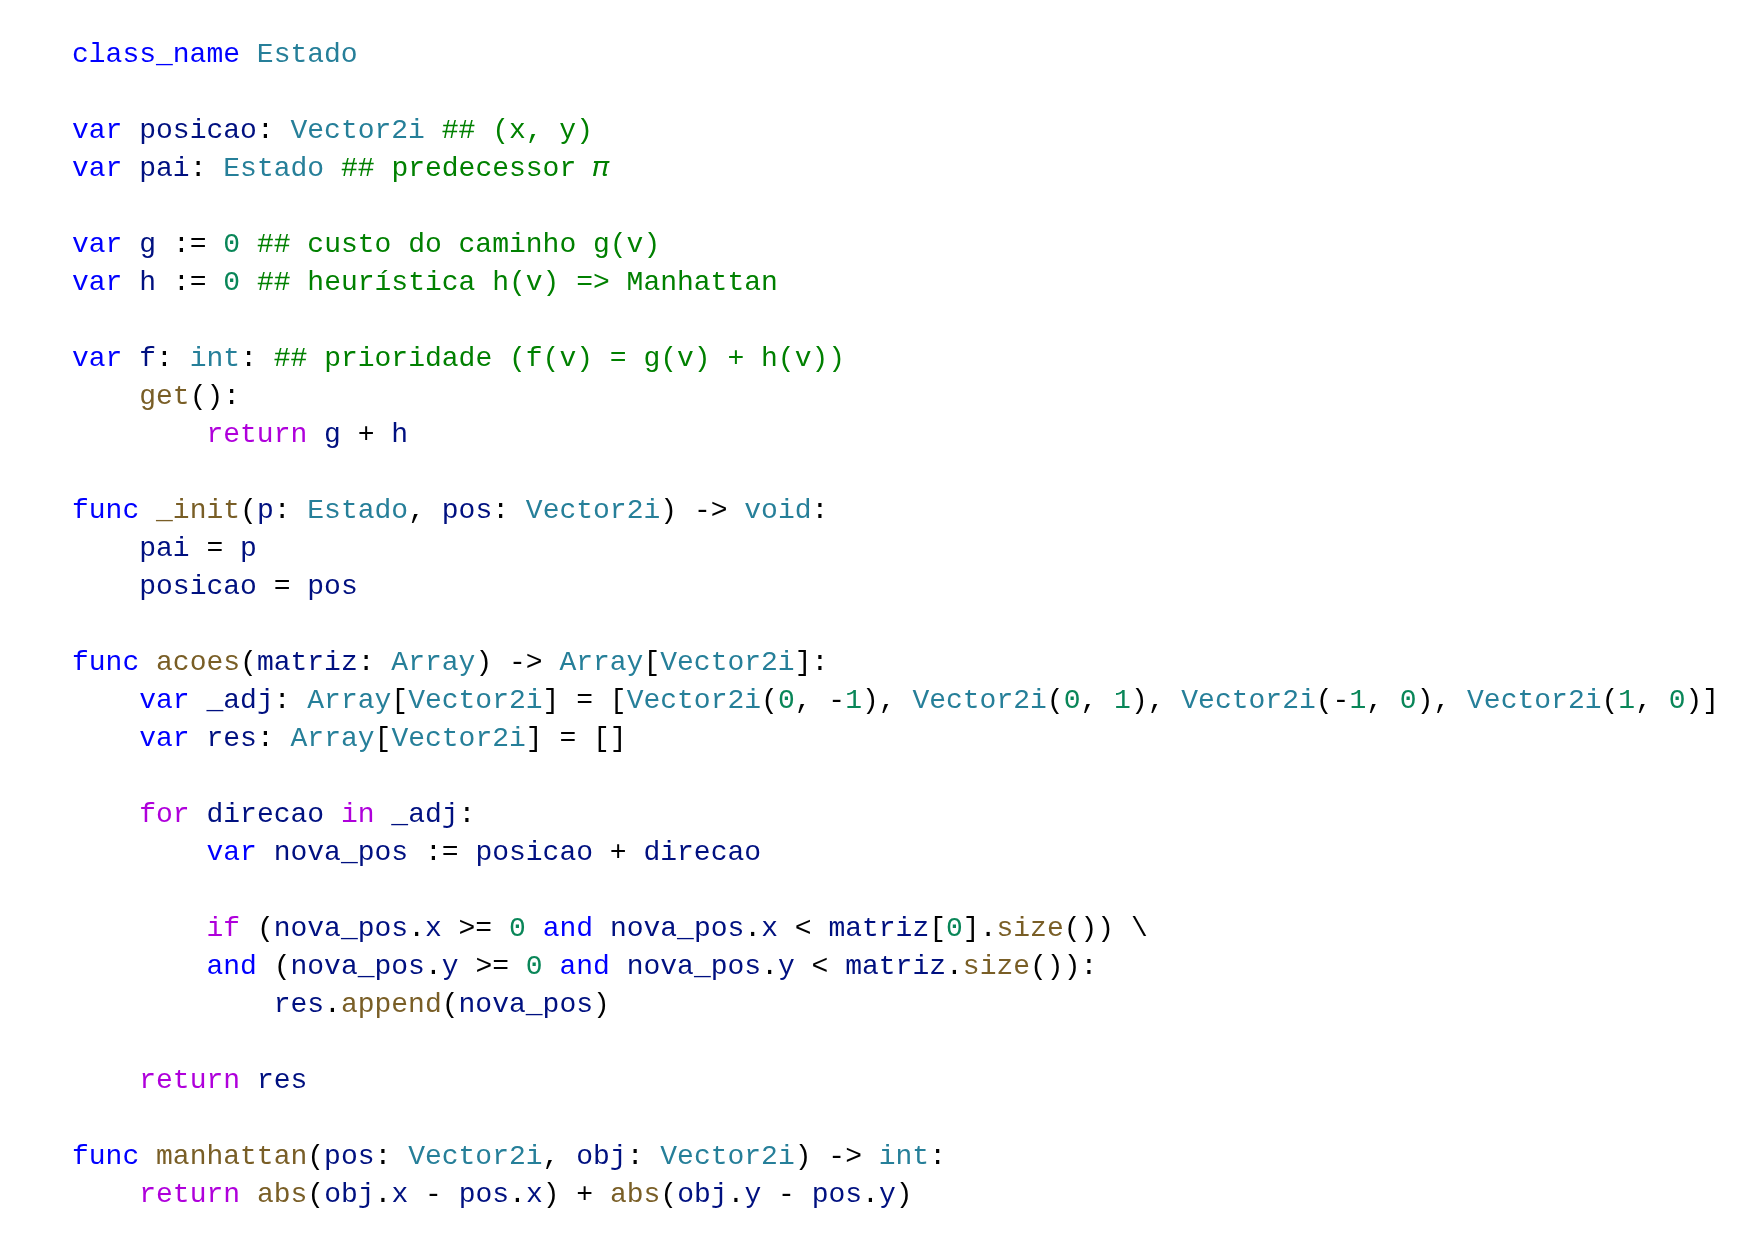
\includegraphics[width=\textwidth]{figuras/scripts/code_estado.png}
    \fonte{Elaborado pelos autores (2026).}
\end{figure}


